\section{Additional Details}

\subsection{Framework Overview}

The end-to-end workflow is: real decode run $\rightarrow$ trace adapter $\rightarrow$ region-level trace $\rightarrow$ virtual PIM replay $\rightarrow$ policy comparison. The framework deliberately separates runtime measurement from the virtual backend so that different cost-model settings can be replayed on the same collected traces.

\subsection{Additional Tables}

The main paper already contains the representative modern-family results table and the family-onset summary table. We do not repeat them here in order to avoid duplicated numbering and cross-reference ambiguity.

\begin{table}[t]
\centering
\caption{Virtual backend inputs grouped by provenance.}
\label{tab:backend-measured-modeled}
\begin{tabular}{p{0.22\linewidth}p{0.37\linewidth}p{0.27\linewidth}}
\toprule
Category & Fields & Source / Interpretation \\
\midrule
Trace-measured & region label, measured latency, context length, batch size & Directly observed in the collected decode traces \\
Trace-derived & bytes moved, FLOPs, arithmetic intensity, estimated KV bytes, KV bytes/token, memory-pressure proxy & Derived from runtime metadata and trace-side estimators \\
Modeled only & roofline compute/memory shares, effective PIM bandwidth/throughput modifiers, transfer/sync overheads, estimated PIM latency & Virtual replay assumptions used only for what-if comparison \\
\bottomrule
\end{tabular}
\end{table}

\begin{table}[t]
\centering
\caption{Default virtual backend parameters, role, and provenance.}
\label{tab:backend-params}
\begin{tabular}{p{0.28\linewidth}p{0.13\linewidth}p{0.24\linewidth}p{0.24\linewidth}}
\toprule
Parameter & Default & Role & Provenance \\
\midrule
GPU peak BW & 1935 GB/s & Roofline anchor for memory time & Prior-work A100-style roofline anchor \\
GPU peak throughput & 312 TFLOP/s & Roofline anchor for compute time & Prior-work A100-style roofline anchor \\
PIM peak BW & 2400 GB/s & Baseline virtual PIM memory rate & Memory-centric default: modestly above GPU BW to encode bandwidth advantage without assuming equal compute \\
PIM peak throughput & 18 TFLOP/s & Baseline virtual PIM compute rate & Conservative low-throughput default to avoid overstating compute-heavy gains \\
Transfer overhead & 0.020 ms & Per-dispatch orchestration cost & Conservative midpoint varied again in preset sensitivity \\
Sync overhead & 0.010 ms & Per-dispatch synchronization cost & Conservative midpoint varied again in preset sensitivity \\
Attention BW bonus & 0.20 & Long-context attention memory modifier & Qualitative prior reflecting stronger KV pressure at long context \\
FC parallelism penalty & 0.25 & MLP parallelism penalty & Deliberate penalty to avoid overstating non-attention and MLP benefit \\
Non-attention penalty & 0.10 & Throughput penalty outside attention & Deliberate penalty to keep non-attention gains conservative \\
\bottomrule
\end{tabular}
\end{table}


\subsection{Robustness Notes}

The sensitivity study changes PIM bandwidth and latency presets while leaving the decode traces fixed. The most robust conclusion is the long-context positive-regime story. Borderline early-onset short-context points are more parameter-sensitive, which is why the main paper phrases them as family-dependent onset evidence rather than as universal short-context gains.

\subsection{Decision-Signal Notes}

The held-out decision-signal study uses workload-level labels derived from whether the realistic online predictor exceeds a $1.05\times$ speedup threshold under the current virtual replay setup. It does not predict real-hardware benefit. Family-held-out evaluation shows that context length is the strongest coarse predictor in the current setup, while attention-only cues are too permissive. Context-bucket-held-out evaluation shows a modest benefit from combining context and KV-related features, which is why the main paper treats KV signals as complementary rather than dominant. Across thresholds from $1.01\times$ to $1.10\times$, the qualitative ordering is unchanged on the current workload set.

\begin{figure}[t]
    \centering
    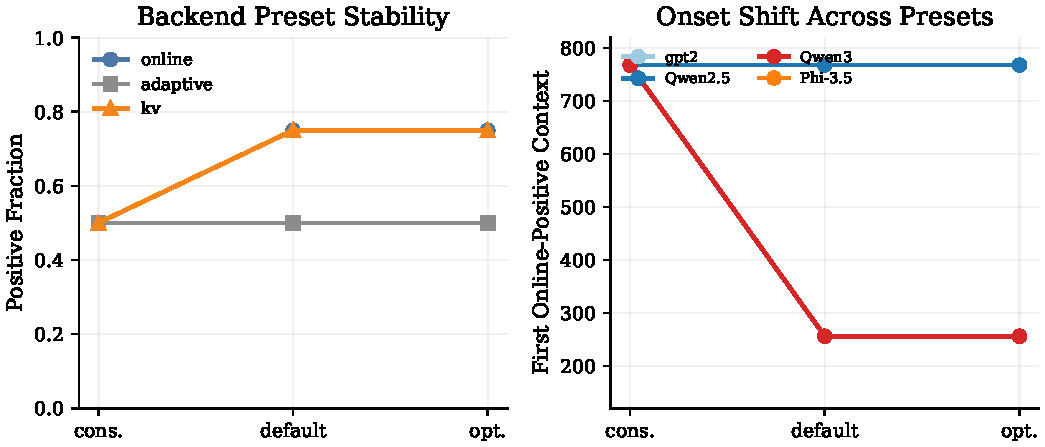
\includegraphics[width=0.95\linewidth]{figures/final_figures/paper_backend_validation.pdf}
    \caption{Appendix robustness view. Left: preset-level positive fractions across conservative/default/optimistic backend settings. Right: first-positive context for representative families across the same presets. Absolute positivity changes, but delayed-onset families remain delayed and early-positive families remain early.}
    \label{fig:backend-validation}
\end{figure}

\subsection{Reproducibility}

All main figures in the paper are generated from reproducible scripts and stored under the project \texttt{final/} package. The trace schema, simulator, cost model, and policy implementations are contained in the repository. The paper focuses on runtime-grounded virtual replay rather than private serving traces or proprietary hardware measurements. The main additional analysis artifacts are \texttt{artifacts/reports/BACKEND\_FORMALIZATION.md}, \texttt{artifacts/reports/DECISION\_SIGNAL\_STUDY.md}, \texttt{artifacts/reports/QUANTIZATION\_VARIATION\_REPORT.md}, and \texttt{artifacts/reports/SAME\_CONTEXT\_FAMILY\_REPORT.md}.
